%
% teil3.tex -- Beispiel-File für Teil 3
%
% (c) 2020 Prof Dr Andreas Müller, Hochschule Rapperswil
%
% !TEX root = ../../buch.tex
% !TEX encoding = UTF-8
%
\subsection{Selektion
\label{buch:paper:varalg:subsection:selection}}
\rhead{Selektion}
In diesem Schritt werden Elternpaare ausgewählt, aus denen neue 
Nachkommen erzeugt werden. Die Selektion erfolgt so, dass in der 
Regel nur die Fittesten die Chance erhalten, neue Kinder zu erzeugen. 
Es gibt jedoch auch die Möglichkeit, dass weniger fitte Individuen die 
Chance haben, neue Nachkommen zu erzeugen, ähnlich wie in der Natur.
Durch die weniger Geeigneten wird die Vielfalt der Population erhalten
und es stellt sicher, dass die Population nicht zu schnell 
konvergiert\footnote{
    Konvergenz bedeutet in diesem Fall, dass die Lösungen mit jeder neuen 
    Population immer ähnlicher zur vorherigen Population werden.
    }
und in einem lokalen Minimum stecken bleibt. Würde dieser Fall eintreten, 
kann es sein, dass wir keine besseren Lösungen erhalten können, obwohl es 
diese gibt. Die Abbildung
\ref{fig:selection_of_parents} veranschaulicht die Selektion.
\begin{figure}
    \centering
    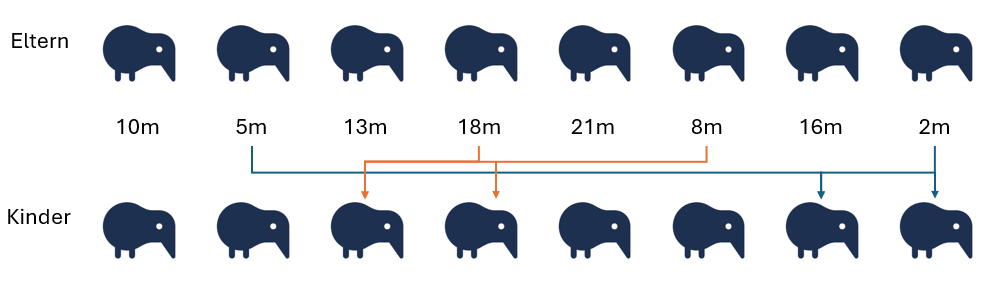
\includegraphics[width=0.8\textwidth]{
        papers/varalg/images/teil3/04OffspringProbability.png
    }
    \caption{
        Mögliche ausgewählte Eltern für Nachkommen, wobei die blaue Linie 
        eine höhere Wahrscheinlichkeit hat, dass diese passiert, als die rote Linie}
    \label{fig:selection_of_parents}
\end{figure}
Für die Selektion gibt es verschiedene Möglichkeiten, die folgenden zeigen bewährte
Methoden auf.
\begin{enumerate}
    \item \textbf{Roulette-Rad-Selektion:} Individuen werden zufällig und
    proportional zu ihrer Fitness ausgewählt. Die Wahrscheinlichkeit wird 
    anhand ihrer Fitness definiert. Die Wahrscheinlichkeit lässt sich mit der Formel
    \begin{equation}
        P_i
        =
        \frac{f_i}{\sum_{j=1}^{N} f_j}
        \label{eq:probability_fittest}
    \end{equation}
    berechnen. In dieser Formel sind hohe Fitnesswerte wahrscheinlicher. Die Funktion \(f_i\) 
    berechnet die Fitness des Individuums. Im Nenner erhalten wir die totale Fitness der Population.
    \item \textbf{Rangselektion:} Individuen werden nach ihrer Fitness sortiert und basierend
    auf ihrem Rang ausgewählt. Die Formel 
    \begin{equation}
        P_i
        =
        \frac{r_i}{\sum_{j=1}^{N} r_j}
        \label{eq:probability_rating}
    \end{equation}
    ist die gleiche wie \eqref{eq:probability_fittest}, mit dem Unterschied, dass die verwendete Funktion 
    \(r_i\) den Rang des Individuums zurückgibt.
    \item \textbf{Turnierselektion:} Eine Gruppe von Individuen wird zufällig ausgewählt
    und das fitteste Individuum dieser Gruppe wird als Elternteil gewählt.
\end{enumerate}
Es gibt auch die Möglichkeit, ein eigenes Selektionssystem zu entwickeln, 
das ein Ausscheidungsverfahren beinhaltet, aus dem schliesslich ein 
Elternpaar hervorgeht. Das System folgt einem logischen Ablauf, wobei 
die Wahrscheinlichkeit mathematisch berechnet wird.

\subsection{Selektion auf das TSP angepasst
\label{buch:paper:varalg:subsection:selection_tsp}}
\rhead{Selektion TSP}
Beim Traveling Salesman Problem sucht man nach der kürzesten Strecke. Die Formel 
\eqref{eq:probability_fittest} würde aber die längste Strecke höher gewichten, was
nicht dem Ziel entspricht. Daher wird die Formel angepasst und neu zu 
\begin{equation}
    P_i
    =
    \frac{\frac{1}{f_i}}{\sum_{j=1}^{N} \frac{1}{f_j}}
    \label{eq:probability_fittest_tsp}
\end{equation}
definiert. Der Term \(\frac{1}{f_i}\) kehrt die Funktion um, sodass kürzere Strecken eine höhere
Wahrscheinlichkeit haben.
